\chapter{Spectra of \prox}
\protect\label{chapter:proxima}
\lhead{Chapter \ref{chapter:proxima}. \emph{Spectra of \prox}}

Two sources of spectra for {\prox} are considered in this study, those from {\uves} taken between 10 and 14 March 2009
studied in \citet{fuhrmeister11} and {\harps} spectra with 260 data points between May 2004 and January 2014 from the
ESO archive\footnote{Based on data obtained from the ESO Science Archive Facility from programs 072.C-0488(E),
  082.C-0718(B), 183.C-0437(A) and 191.C-0505(A).} and referenced in \citet[Table 3]{suarezmascareno15}. The latter were
supplemented with 56 additional spectra from {\harps} taken between 19 January and 30 March 2016\footnote{Based on data obtained
  from the ESO Science Archive Facility from programs 096.C-0082(A) through to 096.C-0082(F).}. The {\uves} data were
obtained with a 0.8/1.10'' slit, yielding a resolution of approximately 60,000., while the resolution of {\harps} is
approximately 120,000. Also studied in Section \ref{section:uvesflares} are the X-ray data from XMM-Newton used in the
\citet{fuhrmeister11} paper\footnote{Provided by Fuhrmeister, priv. comm.} to identify any association between strong
X-ray values and possible corresponding changes to the {\ha} profile.

The bulk of the results from {\harps} in this chapter are taken using the full set of data up to 30 March 2016. However
reference is made to the original set to January 2014 (``Set to 2014'') as this is necessary to reproduce previous
calculations of the rotation period of \prox, in particular the 116.6 days reported by \citet[Table 3]{suarezmascareno15},
 which is not reproducible from the full set. The observation times in the Set to 2014 are used in the modelling results
in Chapter \ref{chapter:modelling} as nearly all the work on the modelling was completed prior to 2016.

\section{{\harps} and {\uves} spectra of \prox}

As mentioned in \citet{mohanty03} and subsequent papers such as \citet{jenkins09} and \citet{barnes14} the spectra of
the later of late \rdwarf s from approximately M5 onward, usually show {\ha} in emission, Several of the \rdwarf s
illustrated in \citet[Fig. 6]{barnes14} additionally show a distinct ``horned'' appearance, due to a certain amount of
self-absorption affecting the centre of the {\ha} peak. {\prox} consistently shows this pattern, which is displayed in
\citet[fig. 14]{fuhrmeister11}. The two \horn s surround a local minimum. As well as the equivalent width of the entire
{\ha} peak, the two \horn s vary in relative size over time on either side of the local minimum, which does not greatly
change in morphology over time. This would appear to be because a more symmetrically-distributed spectral line from the
photosphere is overlaid with plage and chromospheric effects which are asymmetric or localised to regions. These may be
compared with the H, K and Ca II lines discussed in \citet{rauscher06}. The main aim of this {\paperorthesis} is to
study the variations in the line and \horn s via various methods to see if periodicity may be reliably recovered.

\section{{\ha} Line measurements}
\protect\label{section:linemeas}

In Fig. \ref{fig:harpsfirstha}, on the left panel, are shown two example spectra from {\harps} nearly 2 years apart,
clearly showing the changes in the amplitude and shape of the {\ha} line. Fig. \ref{fig:harpsfirstha} also illustrates
the regions used to investigate periodic variability.

The spectra were first normalised by iteratively fitting a cubic polynomial to all the points in all the spectra, apart
from the {\ha} region, then excluding points outside 2 standard deviations above or below the fitted polynomial to
eliminate both emission and absorption lines. With the normalised spectra, the Equivalent Widths, abbreviated to ``EW''
hereafter are calculated. Also calculated is what is herein called the ``Peak Ratio'', abbreviated to ``PR'', defined as
the ratio of the mean values of the two \horn s. The ratio tabulated below is the mean value of the ``red'' \horn, i.e. that
for the longer wavelength, divided by the mean value of the ``blue'' {\horn} (i.e. the ratio of the longer wavelength to
the shorter wavelength \horn). For calculation of the Equivalent Width, values of the flux are interpolated up to the
boundaries of the regions chosen, to minimise integer pixel noise effects. The number of pixels in the regions, as
highlighted in Fig. \ref{fig:harpsfirstha} are either 35 or 36 for the {\ha} region and 11 or 12 for the red {\horn} and
14 or 15 for the blue {\horn} on {\uves}. The corresponding numbers on {\harps} are 98 or 99, 26 or 27 and 27 or 28
respectively. (The number of pixels could vary by one due to differing wavelength corrections caused by the heliocentric
component of the Radial Velocities.)

The {\ha} region for calculation of the Equivalent Width is set to encompass the {\ha} peak and runs from 6561.917{\AA}
to 6563.839\AA) as delineated by the dark red vertical lines. The regions selected for the blue and red \horn s are
shaded in blue and red and run from 6562.072{\AA} to 6562.613{\AA} and 6563.000{\AA} to 6563.517{\AA}
respectively. These regions were chosen to optimise variability in the line profiles. Note that the regions selected for
calculation of the Peak Ratios are not quite the same width, the ``blue'' {\horn} region having a width of 0.541{\AA}
and the ``red'' {\horn} region a width of 0.517\AA. This is because in the observed data the ``red'' {\horn} tends to be
higher but narrower than the ``blue'' \horn. As the Peak Ratio is the ratio of the mean value in the two areas, this
should not be of significance.

In the left panel at the top is displayed the telluric line spectrum for an air mass of 1.4, to which 2.5 has been added
for clarity of display. As demonstrated in \citet[Fig. 1]{reiners15}, the telluric effects are negligible in this
region. (The Gaussian used to simulate {\ha} in that paper is considerably broader than that observed in \prox, so the
telluric line at 6564.2{\AA} can impinge on the former.) All the spectral lines identifiable from the Vienna Atomic Line
Database (VALD) are TiO transitions, with the exception of a MgH line at 6564.29\AA.

In \citet{suarezmascareno15}, the authors use an \textit{{\ha} index}, based in turn upon the work in
\citet{gomesdasilva11}, computed by the formula:

\begin{center}

$ H\alpha_{index} = \frac{H\alpha_{core}}{H\alpha_L + H\alpha_R} $

\end{center}

In this $ H\alpha_{core} $ is defined as the bandpass of width 1.6{\AA} centred on 6562.808{\AA} and $ H\alpha_L $ and
$H \alpha_R $ are defined respectively as continuum bands of widths 10.75{\AA} and 8.75{\AA} centred on 6550.87{\AA} and
6580.31\AA. That $ H\alpha_{core} $ region is delineated by the solid green vertical lines in both parts of
Fig. \ref{fig:harpsfirstha} and the two continuum regions as the green shaded areas in the right-hand panel of the
figure. An important difference between this and calculation of the Equivalent Widths and Peak Ratios is that the
spectra do not have to be normalised for the {\ha} Index calculation as the calculation supplies its own normalisation.

The region chosen for calculation of the {\ha} Equivalent Width in this {\paperorthesis} is slightly wider than that
chosen for the {\ha} index in the \citet{suarezmascareno15}. This was chosen as it appeared on average to encompass the
whole of the {\ha} peak more accurately and better record the variations. It should be remembered that the regions were
chosen from normalised spectra in this {\paperorthesis} but from unnormalised spectra for calculating the {\ha} Index,
which would appear rather different. In practice there was negligible difference between the calculated results for
either method using the two pairs of limits. Adjusting the continuum ranges used for calculation of the {\ha} Index to
cover much wider ranges, including the entire area of that spectral order clear of the {\ha} peak, whilst yielding
different values, the proportionate ranges were very similar and it made negligible difference (less than 0.1\%) to the
periodicity calculations.

\begin{figure}[!htbp]
\begin{center}
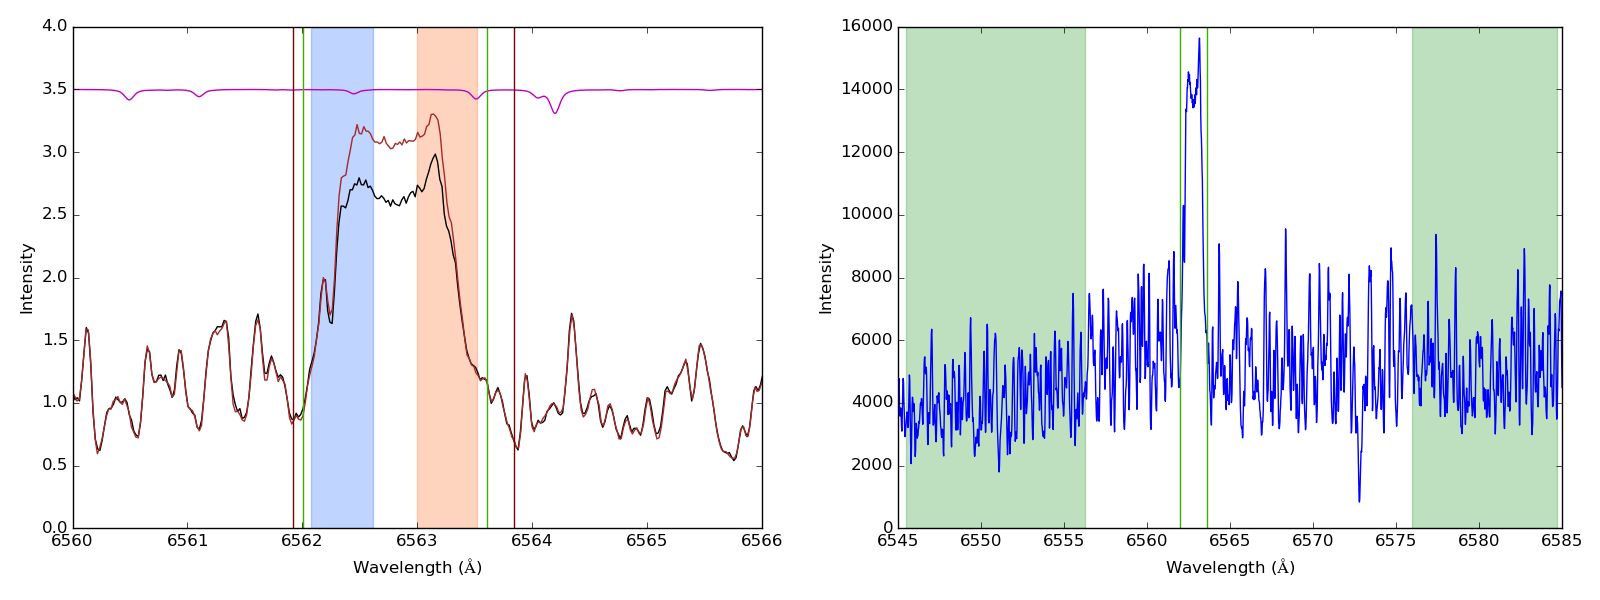
\includegraphics[scale=0.25]{Figures/harpsfirstha4.png} \\
\end{center}   
\caption{In the left panel the {\ha} region of example spectra of {\prox} taken from {\harps} on 27 May 2004 02:10:14
  UTC (black) and 15 March 2006 09:16:35 (brown) are depicted. In the right panel a larger region is selected, just for
  the earlier spectrum in the left panel, however without normalisation. The region delineated with the dark red solid
  vertical lines shows the region used for calculation of the {\ha} equivalent width in this \paperorthesis. The regions
  shaded in red and blue respectively show the regions used for calculation of the sizes of the two \horn s. The solid
  vertical green lines and green shaded areas in the right panel show the regions for calculation of the {\ha} index in
  other papers. The shaded dark green region in the right panel from 6572.468{\AA} to 6573.288{\AA} show the prominent
  TiO I transition line referred to in Section \ref{section:alternativelines}.
}
 \protect\label{fig:harpsfirstha}
\end{figure}

in Table \ref{table:ewtabfirst} are listed the Equivalent Widths, {\ha} Index and Peak Ratios from the {\uves} and
{\harps} data for {\prox}. Histograms of the Equivalent Widths are shown in Fig. \ref{fig:proxhists}. Note
that all the Equivalent Widths from the {\uves} data are displayed, but the seven very highest from the {\harps} data are
omitted, which have Equivalent Widths of over 6, which are listed in Table \ref{table:excessews}.

\begin{table}[!htbp]
\centering
\scalebox{0.75}{
\begin{tabular}{|l|l|l|r|c|c|c|}
\hline
Spectra & From & To & No. & EW & {\ha} Ind & PR \\\hline
\multirow{4}{*}{\uves} & 10/03/2009 & (same) & 215 & 1.759 $ \pm $ 0.301 & 1.759 $ \pm $ 0.301 & 0.850 $ \pm $ 0.021 \\
& 12/03/2009 & (same) & *166 & 1.324 $ \pm $ 0.258 & 1.324 $ \pm $ 0.258 & 0.907 $ \pm $ 0.014 \\
& 14/03/2009 & (same) & 179 & 1.492 $ \pm $ 0.560 & 1.492 $ \pm $ 0.560 & 0.921 $ \pm $ 0.025 \\\cline{2-7}
& \multicolumn{2}{|c|}{ALL} & 560 & 1.570 $ \pm $ 0.428 & 1.570 $ \pm $ 0.428 & 0.899 $ \pm $ 0.036 \\\hline
\multirow{7}{*}{\harps} & 27/05/2004 & 21/07/2004 & 6 & 2.711 $ \pm $ 7.105 & 0.248 $ \pm $ 0.416 & 1.013 $ \pm $ 0.024 \\
& 25/07/2005 & 22/03/2006 & 5 & 1.407 $ \pm $ 0.479 & 0.176 $ \pm $ 0.027 & 0.975 $ \pm $ 0.011 \\
& 14/03/2007 & 19/07/2007 & 5 & 2.012 $ \pm $ 0.542 & 0.210 $ \pm $ 0.031 & 0.999 $ \pm $ 0.010 \\
& 29/06/2008 & 06/04/2010 & 25 & 2.212 $ \pm $ 0.740 & 0.222 $ \pm $ 0.043 & 1.001 $ \pm $ 0.016 \\
& 19/02/2011 & 03/06/2011 & 12 & 2.290 $ \pm $ 4.518 & 0.225 $ \pm $ 0.271 & 0.990 $ \pm $ 0.025 \\
& 18/01/2013 & 10/01/2014 & 207 & 2.004 $ \pm $ 1.004 & 0.210 $ \pm $ 0.059 & 0.994 $ \pm $ 0.017 \\
& 19/01/2016 & 30/03/2016 & 56 & 2.882 $ \pm $ 2.974 & 0.262 $ \pm $ 0.175 & 1.006 $ \pm $ 0.017 \\\cline{2-7}
& \multicolumn{2}{|c|}{All (original set)} & 260 & 2.011 $ \pm $ 1.837 & 0.211 $ \pm $ 0.108 & 0.994 $ \pm $ 0.017 \\
& \multicolumn{2}{|c|}{All (full set)} & 316 & 2.115 $ \pm $ 2.136 & 0.217 $ \pm $ 0.126 & 0.997 $ \pm $ 0.018 \\\hline
\end{tabular}}
\caption{Results for calculation of median and standard deviation {\ha} equivalent widths (EW), {\ha} Index and peak ratio (PR) for {\uves} and
  \harps. In the {\uves} table all the spectra are used and the results shown by day and for all,
  *apart from an observation clearly consisting of noise only timed at
  12/03/09 02:31:11 UTC. In the {\harps} table the observations are separated where they are 300 or more days apart. In
  the summary lines ``original set'' refers to the observations up to 10/01/2014 and the ``full set'' also includes data
  from 19/01/2016 to 30/03/2016.}
\protect\label{table:ewtabfirst}
\end{table}

\begin{figure}[!htbp]
\begin{center}
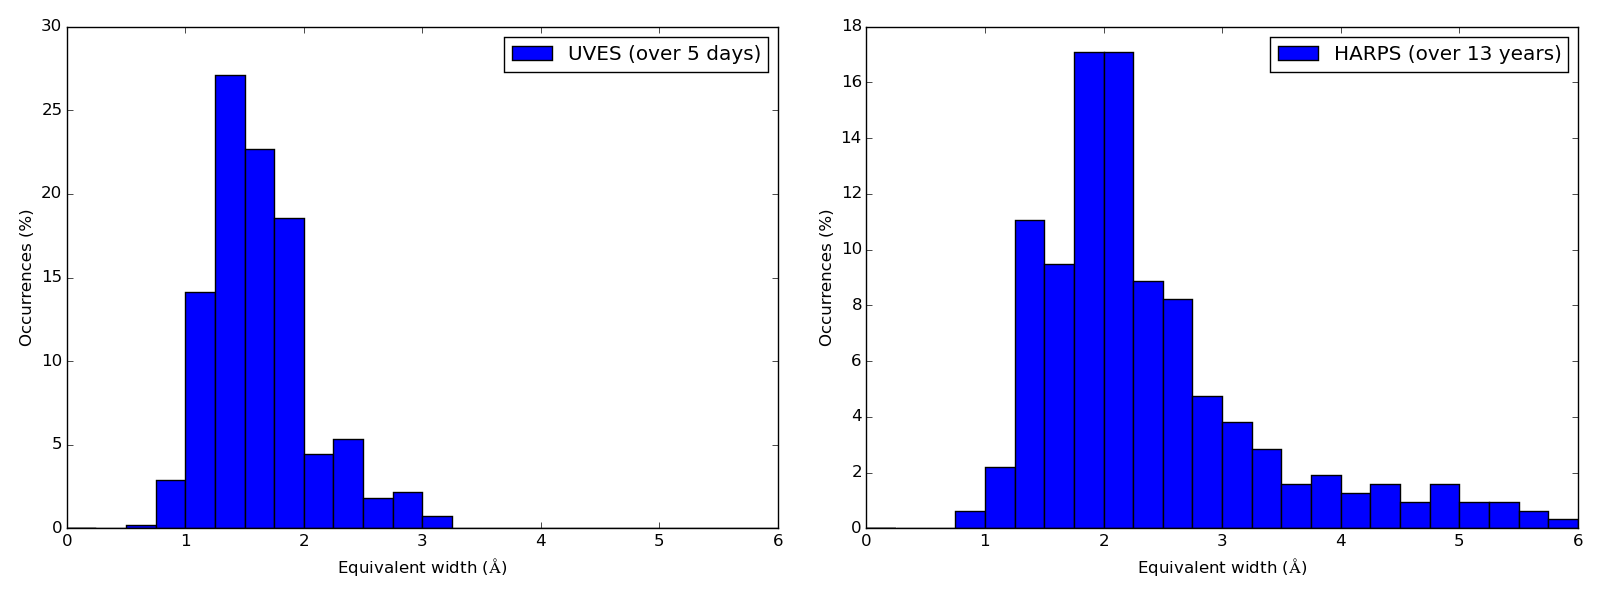
\includegraphics[scale=0.25]{Figures/proxhists.png} \\
\end{center}
\caption{Histogram of equivalent widths for {\uves} on the left and {\harps} on the right with the same X axis
  scale. All the {\uves} spectra results are shown apart from those for one which appeared to be just noise (12
  March 2009 UTC 02:31:11). {\harps} spectra are omitted for four outlying cases which appeared to be dominated by
  flares.}
 \protect\label{fig:proxhists}
\end{figure}
% Done with 25 bins scale 0:6

This {\paperorthesis} investigates calculations of periodicity from skewness, kurtosis and residual {\ha} lines. The residuals were
created by division of each spectrum by the spectrum with the lowest measured Equivalent Width and also the mean of the
5 spectra with the lowest equivalent widths. (See Section \ref{section:harpsper} below). The same two spectra which are
displayed in the left panel of Fig. \ref{fig:harpsfirstha} are re-displayed after this treatment in
Fig. \ref{fig:harpsfirsthad5}.

\begin{figure}[!htbp]
\begin{center}
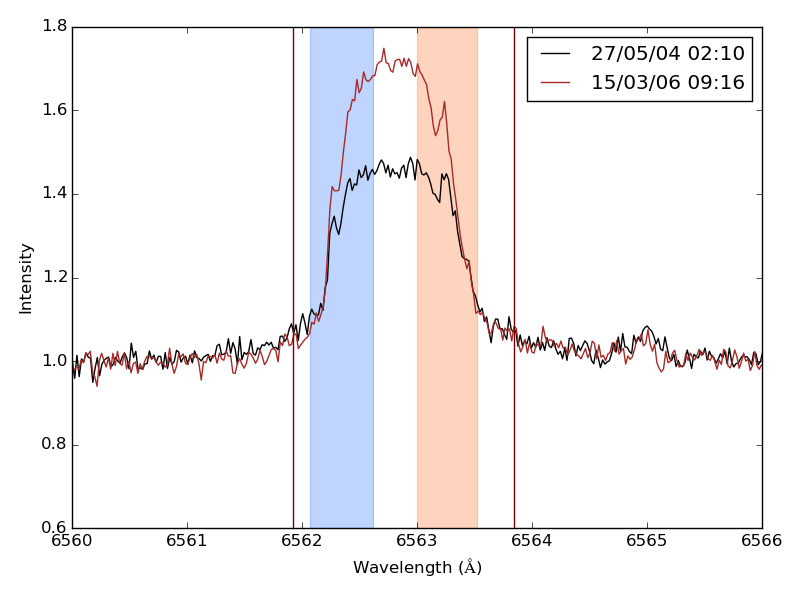
\includegraphics[scale=0.25]{Figures/harpsfirsthad5.png} \\
\end{center}   
\caption{This figure shows the residuals of the same two spectra as previously shown in the left panel of
 Fig. \ref{fig:harpsfirstha} after division by the mean of the first five spectra with minimum equivalent width
timed at 16 March 2006 UTC 06:37:59, 14 March 2007 UTC 07:28:29, 5 April 2011 UTC 03:26:33, 8 April 2011 UTC 06:28:17
and 22 April 2011 UTC 05:07:46.}
\protect\label{fig:harpsfirsthad5}
\end{figure}

\Notnow{
\begin{table}[!htbp]
\centering
\scalebox{0.75}{
\begin{tabular}{|l|l|r|c|c|}
\hline
From & To & No. & EW & PR \\\hline
%\multirow{11}{*}{Div by 1} & 27/05/04 & 21/07/04 & 6 & 1.167 $ \pm $ 4.633 & 1.062 $ \pm $ 0.032 \\\hline
%& 27/05/04 & 21/07/04 & $\dagger$5 & 0.699 $ \pm $ 0.952 & 1.043 $ \pm $ 0.023 \\\cline{2-6}
%& 25/07/05 & 22/03/06 & 5 & 0.346 $ \pm $ 0.290 & 1.016 $ \pm $ 0.014 \\\cline{2-6}
%& 14/03/07 & 19/07/07 & 5 & 0.732 $ \pm $ 0.338 & 1.039 $ \pm $ 0.011 \\\cline{2-6}
%& 29/06/08 & 06/04/10 & 25 & 0.828 $ \pm $ 0.458 & 1.046 $ \pm $ 0.015 \\\cline{2-6}
%& 19/02/11 & 03/06/11 & 12 & 0.877 $ \pm $ 3.005 & 1.037 $ \pm $ 0.027 \\\cline{2-6}
%& 19/02/11 & 03/06/11 & $\dagger$11 & 0.702 $ \pm $ 0.601 & 1.036 $ \pm $ 0.024 \\\cline{2-6}
%& 18/01/13 & 10/01/14 & 207 & 0.702 $ \pm $ 0.643 & 1.040 $ \pm $ 0.018 \\\cline{2-6}
%& 18/01/13 & 10/01/14 & $\dagger$205 & 0.701 $ \pm $ 0.580 & 1.039 $ \pm $ 0.018 \\\cline{2-6}
%& \multicolumn{2}{|c|}{ALL} & 260 & 0.704 $ \pm $ 1.199 & 1.040 $ \pm $ 0.019 \\\cline{2-6}
%& \multicolumn{2}{|c|}{ALL} & $\dagger$256 & 0.702 $ \pm $ 0.581 & 1.039 $ \pm $ 0.018 \\\hline
27/05/04 & 21/07/04 & 6 & 1.020 $ \pm $ 4.401 & 1.051 $ \pm $ 0.032 \\\hline
27/05/04 & 21/07/04 & $\dagger$5 & 0.577 $ \pm $ 0.903 & 1.035 $ \pm $ 0.022 \\\hline
25/07/05 & 22/03/06 & 5 & 0.243 $ \pm $ 0.273 & 1.004 $ \pm $ 0.015 \\\hline
14/03/07 & 19/07/07 & 5 & 0.609 $ \pm $ 0.320 & 1.026 $ \pm $ 0.011 \\\hline
29/06/08 & 06/04/10 & 25 & 0.698 $ \pm $ 0.433 & 1.034 $ \pm $ 0.014 \\\hline
19/02/11 & 03/06/11 & 12 & 0.744 $ \pm $ 2.862 & 1.030 $ \pm $ 0.025 \\\hline
19/02/11 & 03/06/11 & $\dagger$11 & 0.578 $ \pm $ 0.568 & 1.028 $ \pm $ 0.022 \\\hline
18/01/13 & 10/01/14 & 207 & 0.578 $ \pm $ 0.610 & 1.028 $ \pm $ 0.017 \\\hline
18/01/13 & 10/01/14 & $\dagger$205 & 0.577 $ \pm $ 0.550 & 1.028 $ \pm $ 0.017 \\\hline
\multicolumn{2}{|c|}{ALL} & 260 & 0.579 $ \pm $ 1.139 & 1.028 $ \pm $ 0.018 \\\hline
\multicolumn{2}{|c|}{ALL} & $\dagger$256 & 0.578 $ \pm $ 0.550 & 1.028 $ \pm $ 0.017 \\\hline
\end{tabular}}
\caption{This table re-displays the {\harps} spectra as previously shown in Table \ref{table:ewtabfirst} after
  calculating the residual spectra from dividing by the mean values of the 5 spectra with the lowest equivalent
  widths. As before, the rows marked {$\dagger$} show where equivalent   widths of greater  than 2 standard deviations
  from the median are removed and the median and standard deviations recalculated.}
\protect\label{table:divcompar}
\end{table}}

\section{Alternative lines to {\ha}}
\protect\label{section:alternativelines}

Although the {\ha} emission line is by far the strongest line on the {\prox} spectra, for comparison this study includes
some analysis of alternative lines and also with combining lines as suggested in \citet{hall99}, however the Equivalent
Widths, with appropriate scaling as the {\ha} line is so much greater in size than the others, are combined rather than
the fluxes as in that paper.

A prominent absorption line consistent across the spectra was identified to be a TiO transition at 6572.468{\AA} to
6573.288{\AA}, highlighted as the dark green shading in the right panel of Fig. \ref{fig:harpsfirstha}. This is enlarged
in Fig. \ref{fig:tispec}. The Equivalent Widths of this line and also the Peak Ratios from the {\harps} data in the same
manner as for Table \ref{table:ewtabfirst} and the results are shown in Table \ref{table:titable}.

\begin{figure}[!htbp]
\begin{center}
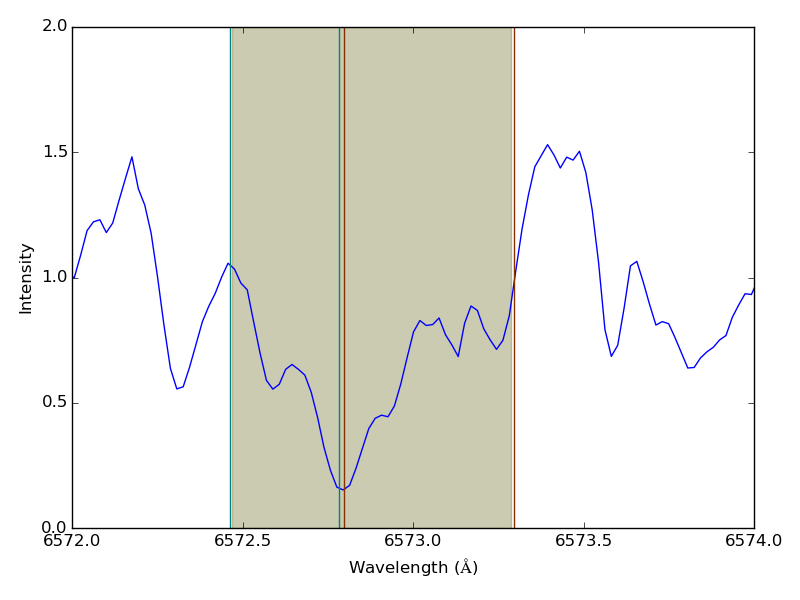
\includegraphics[scale=0.25]{Figures/tispec.png} \\
\end{center}   
\caption{This shows the section of the first spectrum in the {\harps} data (at 27 May 2004 UTC 02:10:14) used for
  calculating Equivalent Widths and also Peak Ratios from the TiO absorption line from 6572.468{\AA} to
  6573.288{\AA}. The blue vertical lines at 6572.463{\AA} and 6572.784{\AA} and the red lines at 6572.797{\AA} and
  6573.295{\AA} delineate the regions used for calculation of Peak Ratios.}
\protect\label{fig:tispec}
\end{figure}

\begin{table}[!htbp]
\centering
\scalebox{0.75}{
\begin{tabular}{|l|l|r|c|c|c|}
\hline
From & To & No. & EW  & Index & PR \\\hline
27/05/2004 & 21/07/2004 & 6 & 0.309 $ \pm $ 0.019 & 0.032 $ \pm $ 0.002 & 1.039 $ \pm $ 0.027 \\
25/07/2005 & 22/03/2006 & 5 & 0.314 $ \pm $ 0.004 & 0.032 & 1.017 $ \pm $ 0.012 \\
14/03/2007 & 19/07/2007 & 5 & 0.310 $ \pm $ 0.006 & 0.032 $ \pm $ 0.001 & 1.030 $ \pm $ 0.036 \\
29/06/2008 & 06/04/2010 & 25 & 0.315 $ \pm $ 0.007 & 0.031 $ \pm $ 0.001 & 1.020 $ \pm $ 0.035 \\
19/02/2011 & 03/06/2011 & 12 & 0.312 $ \pm $ 0.008 & 0.032 $ \pm $ 0.001 & 1.036 $ \pm $ 0.024 \\
18/01/2013 & 10/01/2014 & 207 & 0.310 $ \pm $ 0.006 & 0.032 $ \pm $ 0.001 & 1.047 $ \pm $ 0.027 \\
19/01/2016 & 30/03/2016 & 56 & 0.319 $ \pm $ 0.015 & 0.031 $ \pm $ 0.001 & 1.005 $ \pm $ 0.028 \\\hline
\multicolumn{2}{|c|}{ALL} & 316 & 0.312 $ \pm $ 0.010 & 0.032 $ \pm $ 0.001 & 1.036 $ \pm $ 0.033 \\\hline
\end{tabular}}
\caption{Results for calculation of median and standard deviation of the equivalent widths of the TiO transition at 6572.468{\AA} to
6573.288{\AA} from \harps. The observations are separated where they are 300 or more days apart.}
\protect\label{table:titable}
\end{table}

As Table \ref{table:titable} shows, an ``index'' was also considered along the same lines as the {\ha} Index, but the
size and variations (0.032 $\pm$ 0.001) were far too small to be useful.

\section{Flares on {\uves} data and X-ray values}
\protect\label{section:uvesflares}

In \citet[fig. 1 to fig. 3]{fuhrmeister11} the measured flux for various wavelengths for each of the three observation
nights are presented. In Fig. \ref{fig:uvrxp1} are displayed the {\ha} equivalent width and the X-ray counts for these
nights together with the peak ratios. As the X-ray flux is so much greater on the third day, the third panel is
potentially misleading, so these are re-displayed all to the same scale below in the bottom panel.

\begin{figure}[!htbp]
\begin{center}
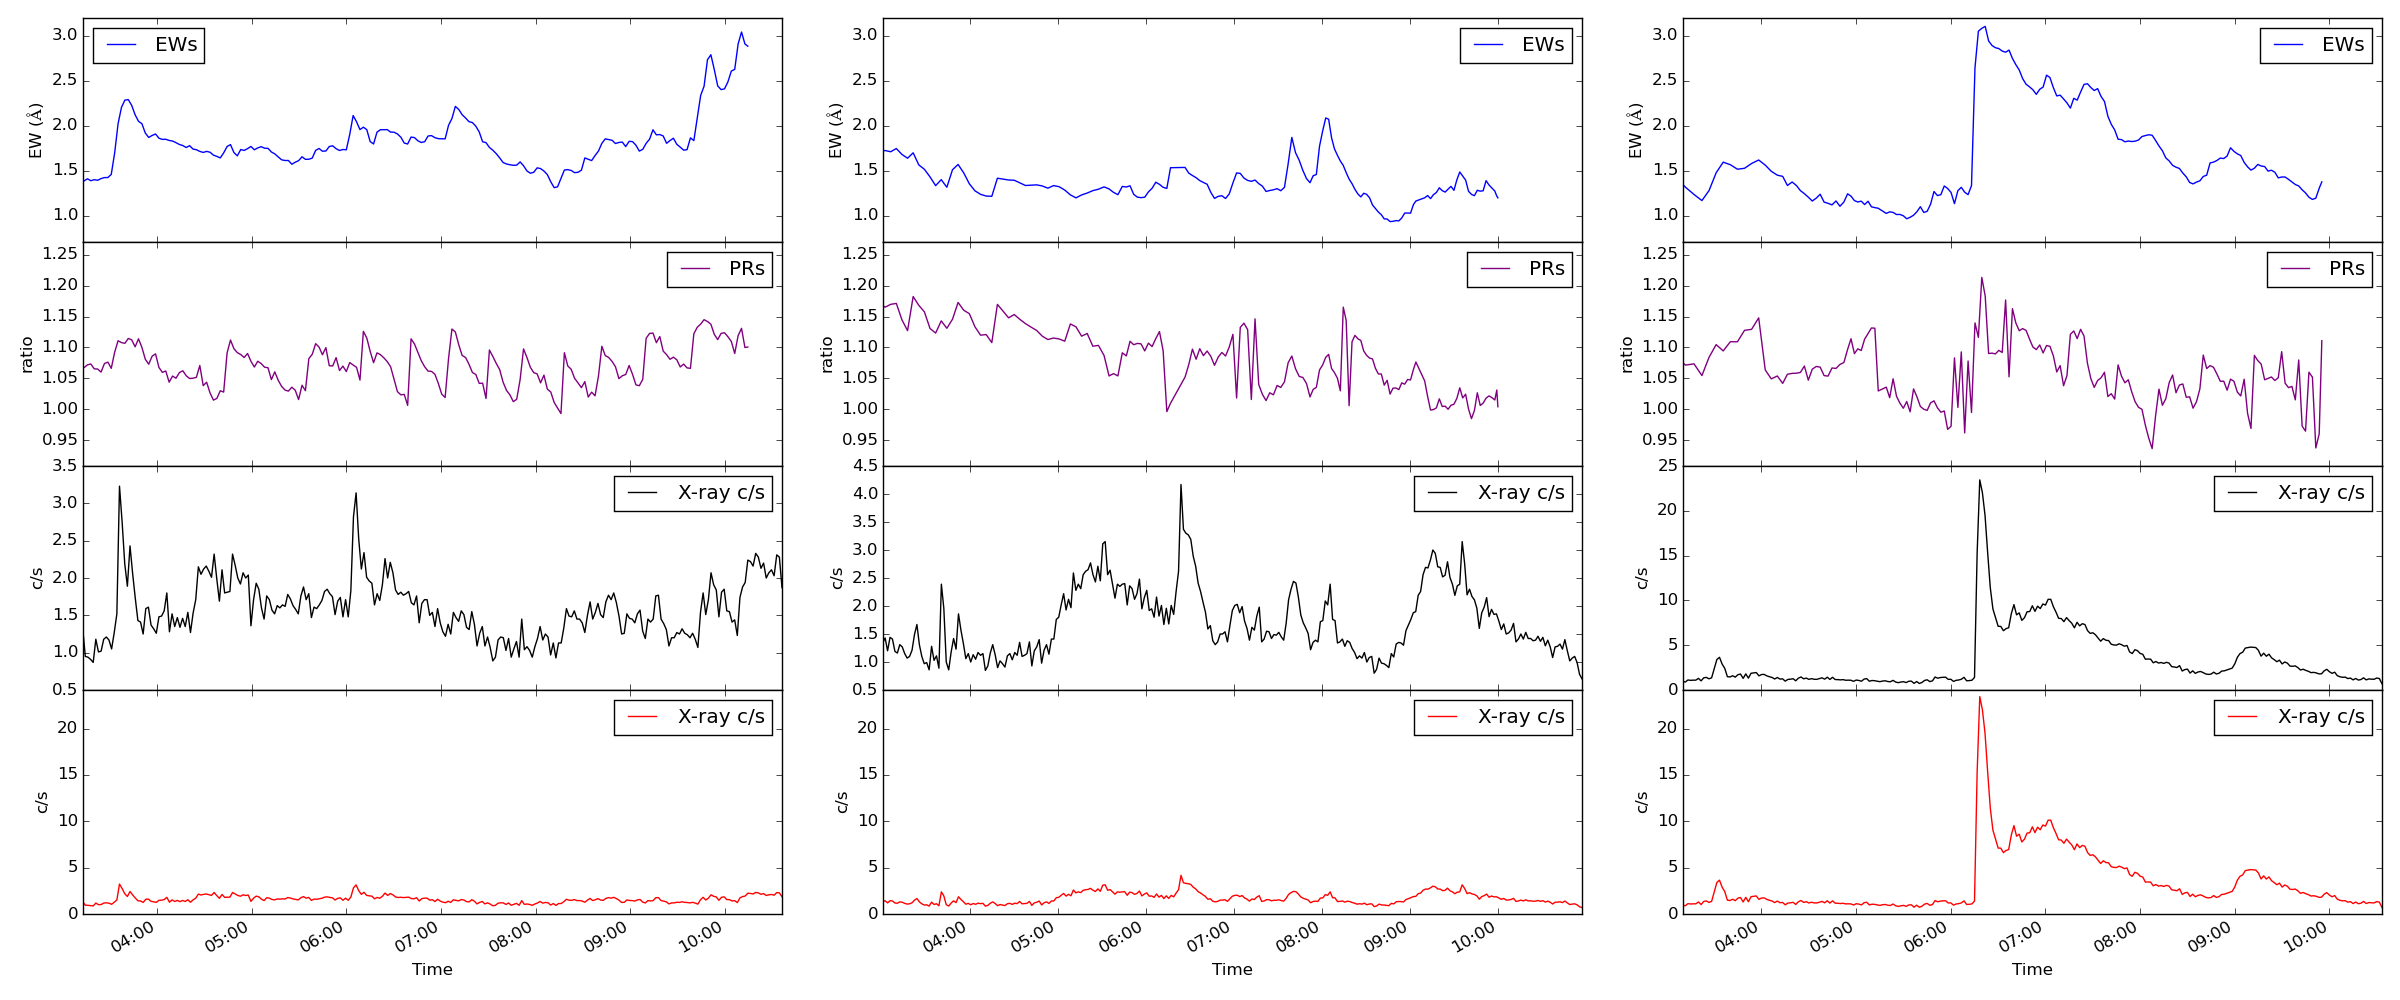
\includegraphics[scale=0.18]{Figures/uvrx-onepic.png} \\
\end{center}   
\caption{The horizontal panels from left to right are for each of the three days of the {\uves} data, 10, 12 and 14
  March 2009.  The Equivalent Width (top panel), Peak Ratio (second panel) and X-ray data (third and bottom panels) of the
  {\ha} flux as shown in \citet[Fig. 1 to Fig.3]{fuhrmeister11}. The top two panels are on the same scale
  throughout. The X-rays displayed are-displayed to the same scale on the fourth panel of each image.}
 \protect\label{fig:uvrxp1}
\end{figure}

In Fig. \ref{fig:uvrxp1} {\Firstp} it is apparrent that the Peak Ratios for the first day (10 March 2009) seemed to have
periodic nature for a portion of the plot, as did a much smaller portion of the plot for the third day (14 March
2009). The portion on the first day had a strong period of approximately half an hour and the third day a much weaker
period of about 20 minutes.  However there were no other periods found in the other day of a similar strength or value,
either for Peak Ratios or Equivalent Widths. However it was noted that in \citet[Section 4.1]{barnes14} there is
speculation of instrumentation error on the first and third days applied to this data. By cross-correlation using the
6565-6585{\AA} region, it is possible to shift the spectra to compensate for apparent radial velocity variations. This
enables the periodic signal to be reduced substantially in the first day's plot and almost completely in the third day's
plot.

%As these periods were not directly relevant to this project, focusing on the rotation period of
%\prox, {\Firstp} decided not to investigate this particular possible behaviour further until appropriate data is
%available.

The {\uves} data showed a large flare during the third of the observation periods starting at approximately 06:15 on
14th March 2009. Both the equivalent width and X-ray counts rapidly reached a peak, with the equivalent width peaking
approximately a minute before the X-ray count peaked. The equivalent width reached a similar level at the end of the
first observation period to that which it reached during the flare in the third, albeit much more slowly, but with only
very slight evidence of a corresponding increase in the X-ray count. However there was an increase in the {\uves}
optical''blue'' flux on the first day, as shown in \citet[fig. 1]{fuhrmeister11} corresponding to the higher Equivalent
Widths suggestive of an alternative temperature.

There is no corresponding X-ray data available for the {\harps} data, but as the {\uves} data suggests that {\ha}
Equivalent Width increases with flares, {\Firstp} selected the higher values of Equivalent Width in the {\harps} data as
indicative of flares. After some experimentation with investigation of periodicity, the effects of possible flares seemed to be
minimised if the proportion of data with the lower 90\% of Equivalent Widths were selected. In both {\uves} and {\harps}
this was approximately one standard deviation from the median, 2.0 in the case of {\uves} and 3.8 in the case of
{\harps}.

The {\harps} data contains seven spectra with particularly large values of Equivalent Width of over 6.000, listed in
Table \ref{table:excessews}.  Following \citet[fig. 8]{fuhrmeister08} in relation to flares on CN Leonis, the He-6678
line Equivalent Widths were also calculated and are also included in that table. It was noticeable that only a few
spectra had any significant He-6678 activity, only seven spectra had Equivalent Widths greater than one standard
deviation of 0.059 above the median of 0.054, which are listed in the table. If these are clipped from the He-6678
results, the standard deviation of the He-6678 line Equivalent Widths sinks to 0.10. In Fig. \ref{fig:dualews} the
Equivalent Widths for {\ha} and He-6678 are plotted against each other for each of the three years 2013, 2014 and
2016, showing the correlation only when the {\ha} line is maximal.

\begin{table}[!htbp]
\centering
\scalebox{0.75}{
\begin{tabular}{|l|r|r|}
\hline
Epoch & \multicolumn{1}{|c|}{EW} & He-6678 \\\hline
18/03/2016 UTC 08:59:02 & 23.991 & 0.853 \\
16/07/2004 UTC 01:52:40 & 21.693 & 0.312 \\
27/03/2011 UTC 05:20:09 & 18.123 & 0.591 \\
31/01/2016 UTC 08:51:35 & 7.298 & *0.099 \\
26/02/2016 UTC 09:07:05 & 6.898 & *0.110 \\
05/05/2013 UTC 03:31:16 & 6.756 & 0.276 \\
05/05/2013 UTC 03:41:47 & 6.192 & 0.177 \\\hline
14/05/2013 UTC 06:07:49 & $\dagger$5.425 & 0.115 \\
05/05/2013 UTC 03:53:13 & $\dagger$5.786 & 0.114 \\\hline
\end{tabular}}
\caption{The seven spectra with Equivalent Widths over 6.000, in descending order, also showing the values of the
  Equivalent Width and that of the He-6678 absorption line. Five spectra have the one of the seven strongest {\ha} lines
  and also one of the seven strongest {\ha} lines. The two He-6678 Equivalent Widths marked with * are where the spectra
  have one of the seven strongest {\ha} lines but are not in the seven strongest He-6678 lines and vice versa for the
  two lines at the bottom of the table marked with $\dagger$.}
\protect\label{table:excessews}
\end{table}

\begin{figure}[!htbp]
\begin{center}
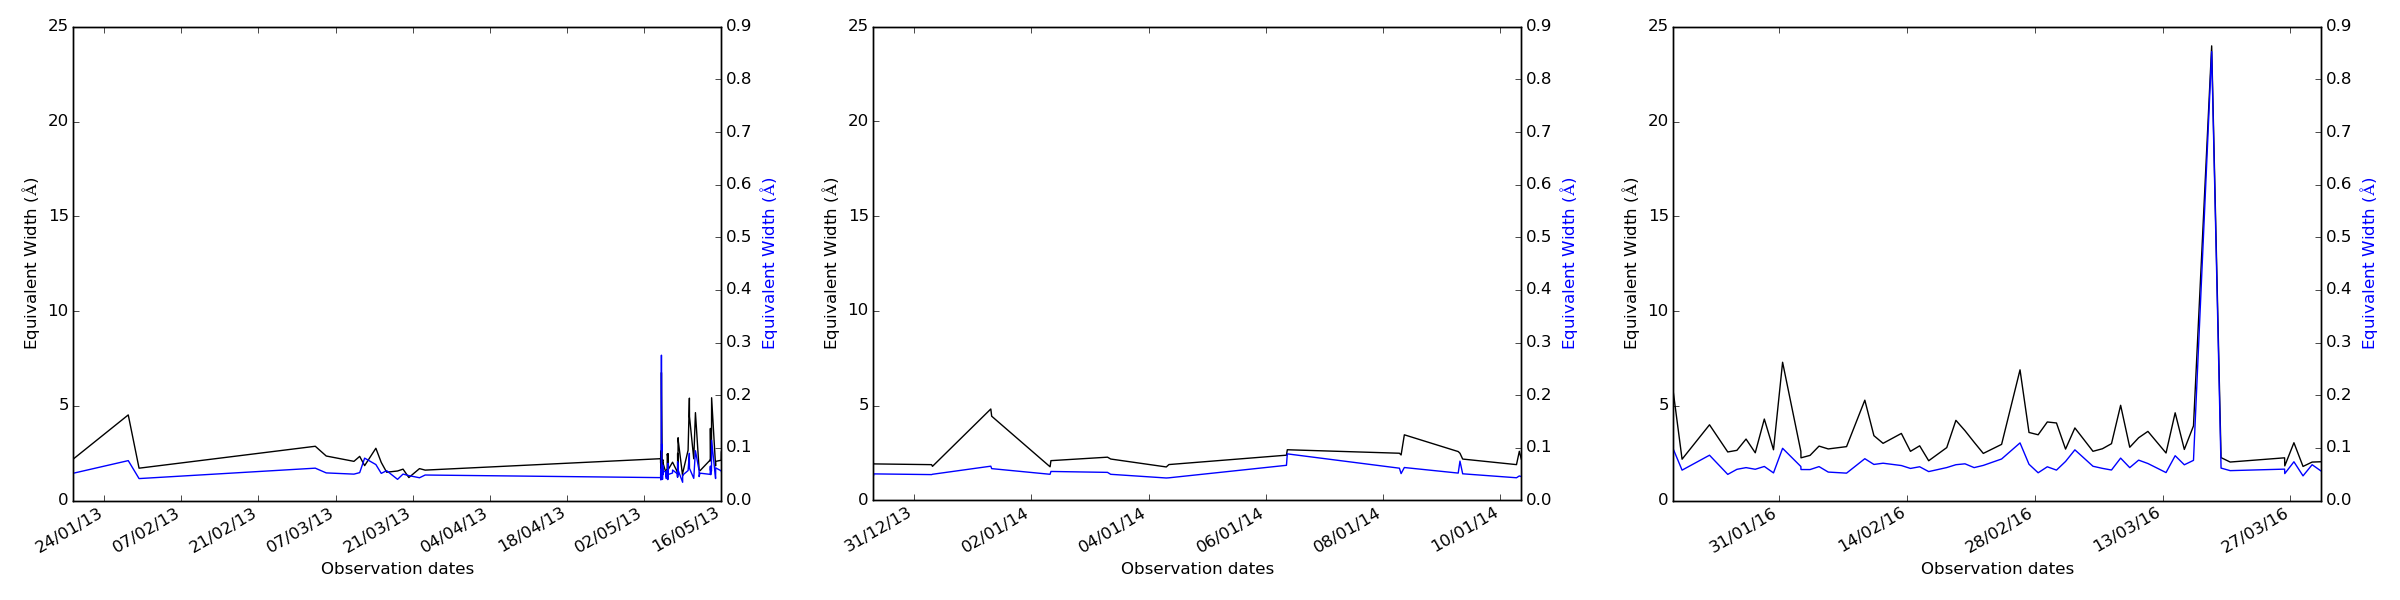
\includegraphics[scale=0.18]{Figures/dualcomb.png} \\
\end{center}   
\caption{The plots show the {\ha} Equivalent Width in black and the He-6678 Equivalent Widths in blue for the {\harps}
  observations in the years 2013, 2014 and 2015. Vertical scales for {\ha} and for He-6678 are the same in each plot.}
 \protect\label{fig:dualews}
\end{figure}
